\section{Phase 2 Results: Graph Attention and the Hybrid}
\label{sec:p2results}
All numbers below are on the test period (4--27 June 2012), which was used once,
after every design decision. Every model receives the same 12-step history and is
scored with the same missing-target mask.

\subsection{The gap exists}
\label{sec:p2gap}
Fig.~\ref{fig:gap} tests the premise of Section~\ref{sec:gap} on out-of-fold
\emph{training} residuals of the per-segment XGBoost models. First, the errors of
road-adjacent segments are correlated: 0.13 at 15\,min and 0.21 at 60\,min, against
0.02 and 0.04 for non-adjacent pairs, and the correlation decays with road distance
(left panel). Second, information available at forecast time that the per-segment
model never received predicts its error. The mean absolute correlation of the
15-minute residual with the \emph{downstream} anomaly is 0.12 and with the upstream
anomaly 0.08, against 0.06 with the segment's \emph{own} anomaly, which the model did
use (right panel). By Eq.~\eqref{eq:gap}, an independent model therefore leaves
accuracy on the table, and the missing information is exactly the state of the
neighbouring links.

\begin{figure}[t]
\centering
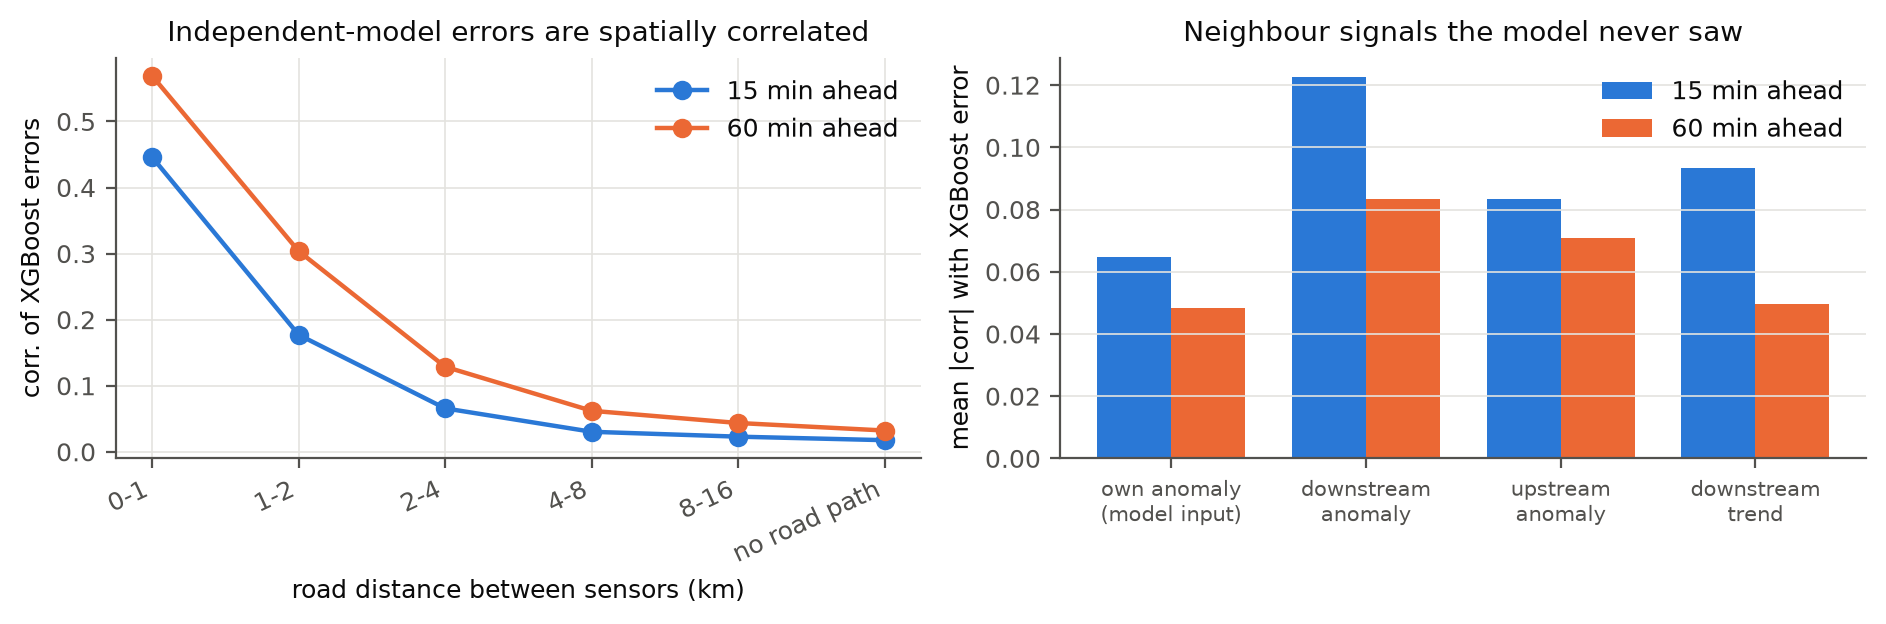
\includegraphics[width=\columnwidth]{p2_gap_analysis.png}
\caption{The gap of independent segment models, on out-of-fold training residuals.
Left: correlation of XGBoost errors between sensor pairs by road distance. Right:
mean $|$correlation$|$ of the error with signals at forecast time.}
\label{fig:gap}
\end{figure}

\subsection{Overall accuracy}
\begin{table*}[t]
\centering
\caption{Test-set accuracy on METR-LA (12-step history for every model). Best of our models in bold. $^\dagger$As reported by Wu et al. (2019).}
\label{tab:p2main}
\setlength{\tabcolsep}{3.5pt}
\begin{tabular}{lccccccccc}
\toprule
 & \multicolumn{3}{c}{15 min} & \multicolumn{3}{c}{30 min} & \multicolumn{3}{c}{60 min} \\ \cmidrule(lr){2-4} \cmidrule(lr){5-7} \cmidrule(lr){8-10}
Model & MAE & RMSE & MAPE\% & MAE & RMSE & MAPE\% & MAE & RMSE & MAPE\% \\
\midrule
Historical Average & 4.19 & 7.85 & 13.03 & 4.19 & 7.85 & 13.03 & 4.19 & 7.85 & 13.03 \\
Persistence & 3.50 & 6.42 & 8.61 & 4.21 & 8.05 & 10.85 & 5.38 & 10.34 & 14.52 \\
Ridge (features) & 3.37 & 5.71 & 8.93 & 3.78 & 6.60 & 10.59 & 4.09 & 7.33 & 12.03 \\
Gradient Boosting (features) & 2.89 & 5.56 & 7.79 & 3.29 & 6.54 & 9.43 & 3.66 & 7.45 & 11.13 \\
XGBoost per segment & 2.89 & 5.67 & 8.14 & 3.26 & 6.62 & 9.71 & 3.64 & 7.50 & 11.35 \\
Graph WaveNet & \textbf{2.72} & \textbf{5.18} & \textbf{7.02} & 3.10 & \textbf{6.24} & \textbf{8.52} & 3.59 & 7.42 & \textbf{10.35} \\
ST-GAT & 2.74 & 5.23 & 7.45 & \textbf{3.08} & 6.26 & 8.88 & \textbf{3.47} & \textbf{7.30} & 10.58 \\
Hybrid XGB$\to$GAT & 2.72 & 5.23 & 7.22 & 3.09 & 6.29 & 8.77 & 3.52 & 7.35 & 10.57 \\
\midrule
\multicolumn{10}{l}{\emph{Published results (same data and protocol)}} \\
DCRNN [Li et al. 2018] & 2.77 & 5.38 & 7.30 & 3.15 & 6.45 & 8.80 & 3.60 & 7.60 & 10.50 \\
STGCN [Yu et al. 2018]$^\dagger$ & 2.88 & 5.74 & 7.62 & 3.47 & 7.24 & 9.57 & 4.59 & 9.40 & 12.70 \\
Graph WaveNet [Wu et al. 2019] & 2.69 & 5.15 & 6.90 & 3.07 & 6.22 & 8.37 & 3.53 & 7.37 & 10.01 \\
GMAN [Zheng et al. 2020] & 2.80 & 5.55 & 7.41 & 3.12 & 6.49 & 8.73 & 3.44 & 7.35 & 10.07 \\
\bottomrule
\end{tabular}
\end{table*}

Table~\ref{tab:p2main} and Fig.~\ref{fig:p2horizon} give the full comparison.
\textbf{Both network-aware models clearly beat the independent segment models.}
ST-GAT lowers the average MAE of XGBoost per segment from 3.20 to 3.04\,mph
($-5.0\,\%$; $-5.3\,\%$ at 15\,min, $-4.6\,\%$ at 60\,min), and the hybrid to
3.06\,mph ($-4.5\,\%$). Diebold--Mariano tests reject equal accuracy at every
horizon with $p<0.001$ (Table~\ref{tab:p2dm}), and the hybrid is more accurate than
XGBoost at 79\,\% of the sensors at 60\,min, most strongly along the congested
central corridor (Fig.~\ref{fig:p2improve}). The two independent tabular models are
close to each other (3.20 vs.\ 3.22\,mph), so the gain comes from the network, not
from a better tabular learner.

\textbf{Among the network models the ranking depends on the horizon.} The hybrid is
the most accurate of our models at 15\,min (2.72\,mph), significantly better than
ST-GAT ($p=0.001$), because the per-segment XGBoost supplies a strong short-term level.
At 30 and 60\,min ST-GAT is significantly better than the hybrid ($p<0.01$). ST-GAT
is also the best model at 60\,min overall (3.47\,mph, against 3.59 for Graph WaveNet,
$p<0.001$) with about half the parameters (164k vs.\ 301k). Graph WaveNet keeps a small
but significant edge at 15\,min (2.72 vs.\ 2.74) and the lowest MAPE, which weights
low-speed targets heavily. Our ST-GAT is comparable to published
results under the same protocol (Table~\ref{tab:p2main}, bottom): at 60\,min it is
below DCRNN (3.60) and the published Graph WaveNet (3.53) and close to GMAN (3.44).

Uncertainty across days is large: the 95\,\% day-block bootstrap intervals of average
MAE are $[2.85, 3.16]$ for ST-GAT, $[2.87, 3.18]$ for the hybrid and $[2.99, 3.35]$
for XGBoost per segment. They overlap because some test days are much harder than
others for \emph{every} model. The Diebold--Mariano tests compare the models on the
same forecast times and are therefore far more sensitive to the paired difference.

\begin{figure}[t]
\centering
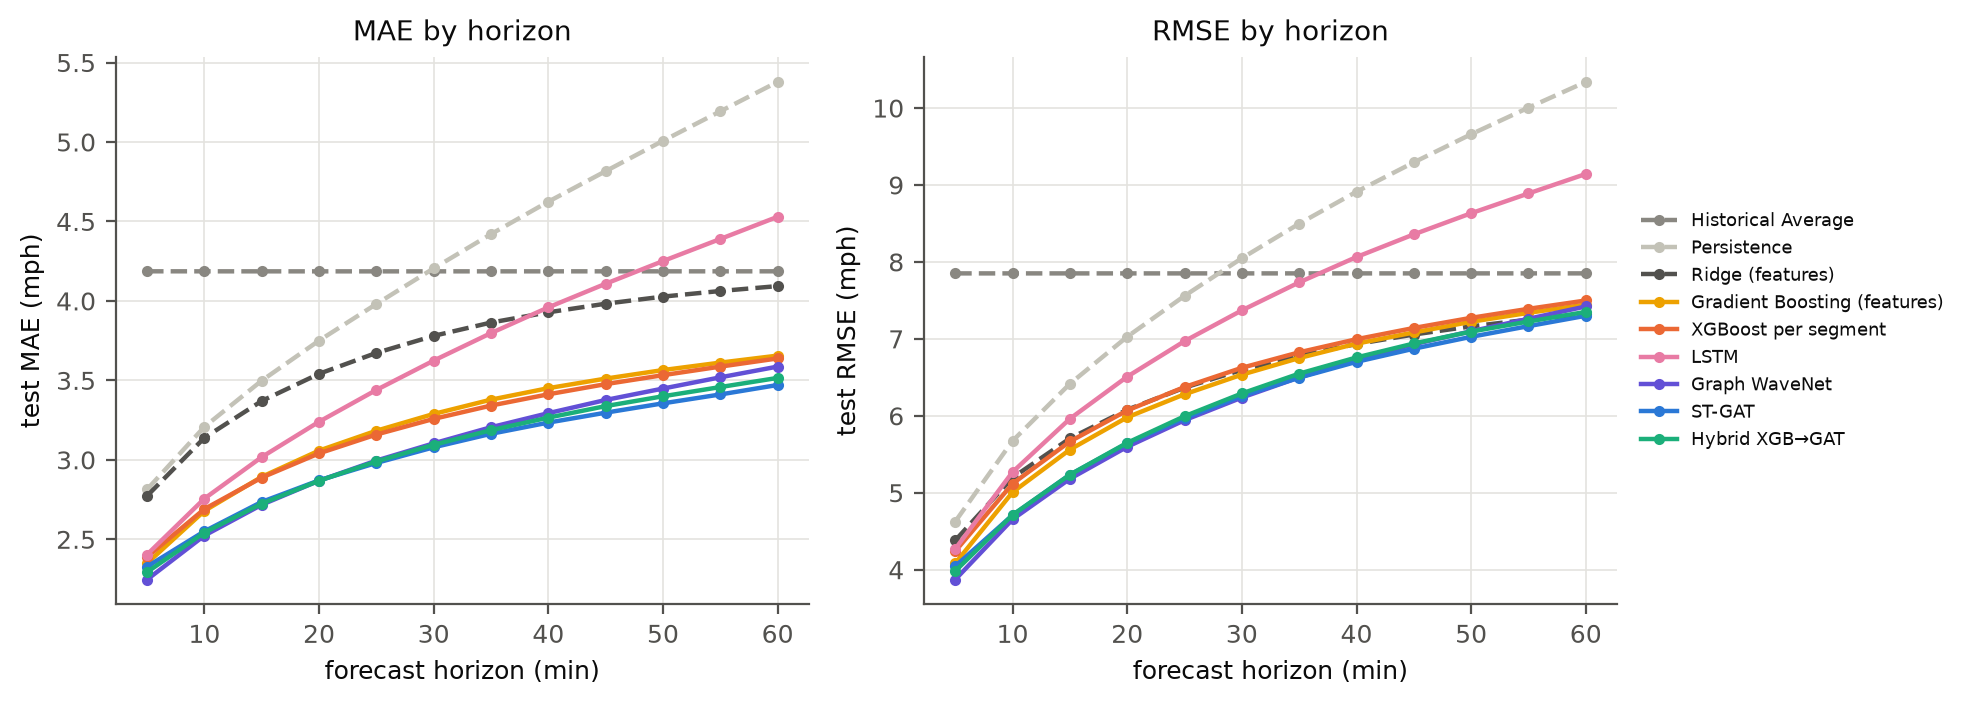
\includegraphics[width=\columnwidth]{p2_horizon_metrics.png}
\caption{Test MAE and RMSE at all 12 horizons. Dashed lines: simple baselines.}
\label{fig:p2horizon}
\end{figure}

\begin{table*}[t]
\centering
\caption{Diebold--Mariano statistic ($p$-value) on absolute error with Newey--West variance. Negative: A is more accurate.}
\label{tab:p2dm}
\setlength{\tabcolsep}{3.5pt}
\begin{tabular}{lccc}
\toprule
Comparison (A vs.\ B) & 15 min & 30 min & 60 min \\
\midrule
Hybrid XGB$\to$GAT vs.\ XGBoost per segment & -25.2 ($<$.001) & -17.2 ($<$.001) & -9.8 ($<$.001) \\
ST-GAT vs.\ XGBoost per segment & -23.5 ($<$.001) & -17.6 ($<$.001) & -11.8 ($<$.001) \\
Hybrid XGB$\to$GAT vs.\ ST-GAT & -3.2 (0.001) & 2.7 (0.008) & 5.0 ($<$.001) \\
ST-GAT vs.\ Gradient Boosting (features) & -27.8 ($<$.001) & -22.2 ($<$.001) & -14.2 ($<$.001) \\
Hybrid XGB$\to$GAT vs.\ Gradient Boosting (features) & -29.2 ($<$.001) & -20.8 ($<$.001) & -12.0 ($<$.001) \\
XGBoost per segment vs.\ Gradient Boosting (features) & -1.1 (0.261) & -5.5 ($<$.001) & -2.1 (0.033) \\
\bottomrule
\end{tabular}
\end{table*}

\subsection{Peak, off-peak and congestion}
\begin{table*}[t]
\centering
\caption{Test MAE (mph) in peak periods (weekdays 06--10 and 15--19, by target time; 25\% of windows) and off-peak, and on congested targets ($<$40\,mph).}
\label{tab:p2regime}
\setlength{\tabcolsep}{3.5pt}
\begin{tabular}{lccccccc}
\toprule
 & \multicolumn{3}{c}{Peak} & \multicolumn{3}{c}{Off-peak} & Congested \\ \cmidrule(lr){2-4}\cmidrule(lr){5-7}\cmidrule(lr){8-8}
Model & 15 & 30 & 60 & 15 & 30 & 60 & 60 min \\
\midrule
Historical Average & 6.04 & 6.04 & 6.04 & 3.51 & 3.51 & 3.51 & 12.90 \\
Persistence & 4.39 & 5.59 & 7.45 & 3.17 & 3.70 & 4.62 & 13.42 \\
Ridge (features) & 4.36 & 5.09 & 5.65 & 3.01 & 3.30 & 3.52 & 11.24 \\
Gradient Boosting (features) & 3.77 & 4.50 & 5.15 & 2.57 & 2.85 & 3.11 & 11.33 \\
XGBoost per segment & 3.82 & 4.49 & 5.19 & 2.54 & 2.81 & 3.07 & 11.79 \\
LSTM & 4.06 & 5.19 & 6.91 & 2.64 & 3.05 & 3.66 & 14.16 \\
Graph WaveNet & 3.53 & 4.24 & 5.12 & \textbf{2.42} & 2.69 & 3.03 & \textbf{10.14} \\
ST-GAT & 3.57 & 4.19 & \textbf{4.88} & 2.43 & \textbf{2.67} & \textbf{2.96} & 10.66 \\
Hybrid XGB$\to$GAT & \textbf{3.50} & \textbf{4.16} & 4.94 & 2.44 & 2.70 & 2.99 & 10.74 \\
\bottomrule
\end{tabular}
\end{table*}
The gains concentrate where traffic is hard (Table~\ref{tab:p2regime},
Fig.~\ref{fig:peak}). In peak periods at 60\,min, ST-GAT lowers XGBoost's MAE from
5.19 to 4.88\,mph ($-6.0\,\%$), against $-3.6\,\%$ off-peak (3.07$\to$2.96). On
congested targets ($<$40\,mph) all graph models cut the 60-minute error of the
independent model by roughly 1--1.6\,mph (11.79$\to$10.14--10.74), which is what
propagation along the road graph should buy. Graph WaveNet is the best model on
congested targets, while ST-GAT is best in free flow; the learned dense adjacency
of Graph WaveNet seems to help most in the rare, severe events, at the price of
slightly worse free-flow accuracy.

\begin{figure}[t]
\centering
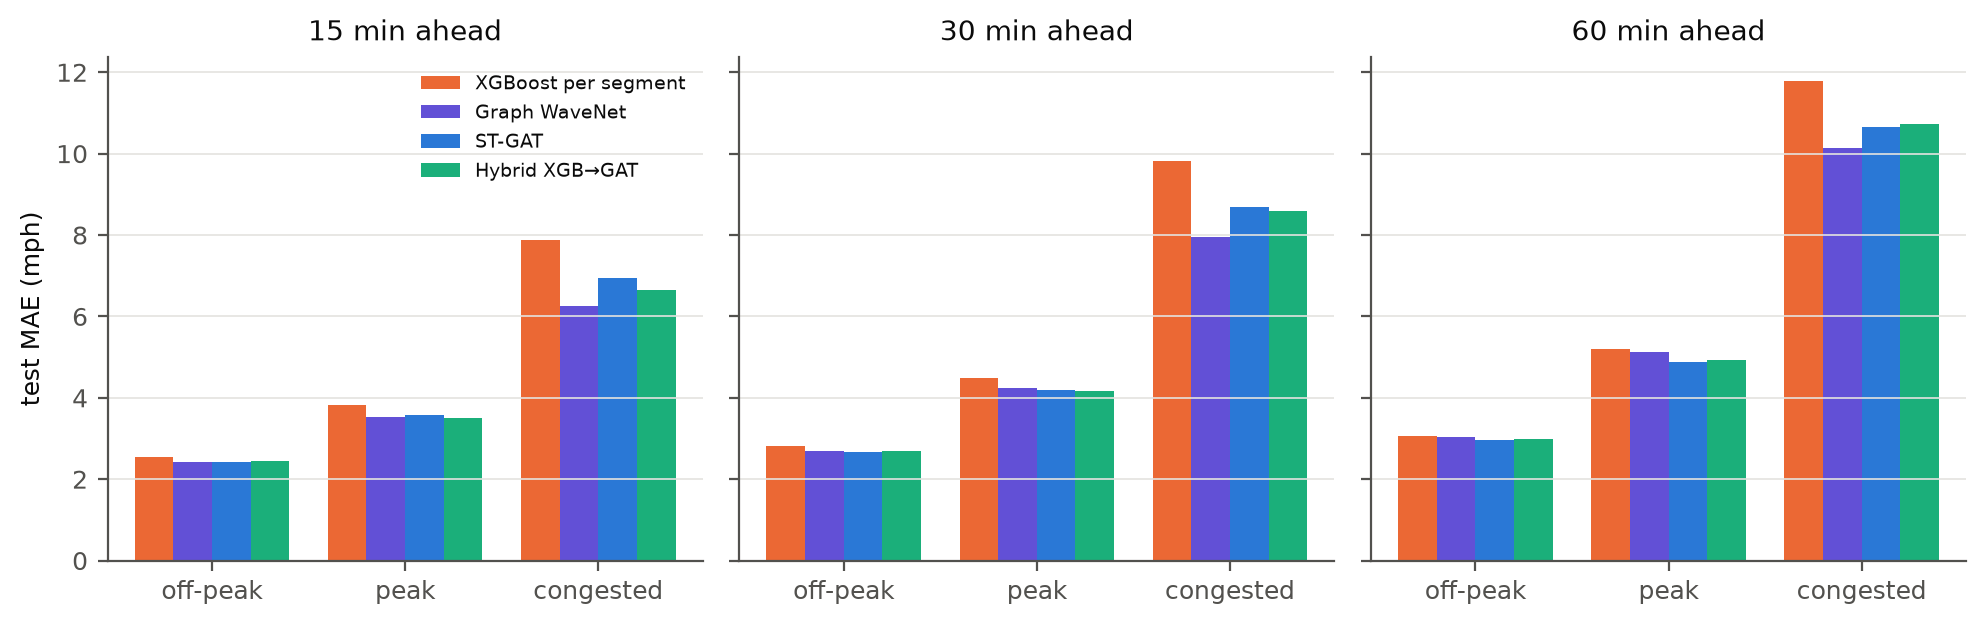
\includegraphics[width=\columnwidth]{p2_peak_offpeak.png}
\caption{Test MAE off-peak, in peak periods (weekdays 06--10 and 15--19) and on
congested targets.}
\label{fig:peak}
\end{figure}

\subsection{Outage robustness}
\begin{table}[t]
\centering
\caption{Robustness to sensor outages: test MAE at 60\,min when the sensor's most recent input reading is observed or missing (12.1\% of cases).}
\label{tab:p2robust}
\setlength{\tabcolsep}{3.5pt}
\begin{tabular}{lccc}
\toprule
Model & Latest observed & Latest missing & Change \\
\midrule
Historical Average & 4.17 & 4.70 & +13\% \\
Persistence & 5.31 & 7.89 & +49\% \\
Ridge (features) & 4.06 & 5.23 & +29\% \\
Gradient Boosting (features) & 3.63 & 4.50 & +24\% \\
XGBoost per segment & 3.61 & 4.75 & +32\% \\
Graph WaveNet & 3.54 & 5.36 & +52\% \\
ST-GAT & 3.44 & 4.41 & +28\% \\
Hybrid XGB$\to$GAT & 3.48 & 4.66 & +34\% \\
\bottomrule
\end{tabular}
\end{table}
Masking outages instead of feeding them as 0\,mph (Section~\ref{sec:dldata}) fixes
the weakness found in Phase~1 (Table~\ref{tab:p2robust}). When a sensor's latest
reading is missing, Graph WaveNet's 60-minute MAE rises by 52\,\%, ST-GAT's by only
28\,\%, which is in line with the forward-filled tabular models (24--32\,\%).

\subsection{Ablations}
\label{sec:p2abl}
All ablation variants are trained for the same 12 epochs (each on a random half of
the training windows) with the same seed, and the full model is retrained under that
budget, so the rows are directly comparable. The completed ST-GAT ablations so far:

\begin{table}[t]
\centering
\caption{ST-GAT ablation (completed variants): test MAE (mph), identical 12-epoch
budget and seed.}
\label{tab:p2abl_partial}
\setlength{\tabcolsep}{3.5pt}
\begin{tabular}{lcccc}
\toprule
Variant & 15 min & 30 min & 60 min & Avg \\
\midrule
Road-graph attention (full) & \textbf{2.76} & \textbf{3.13} & \textbf{3.53} & \textbf{3.08} \\
Mean aggregation (no attention) & 2.76 & 3.14 & 3.55 & 3.10 \\
No spatial module & 2.86 & 3.25 & 3.71 & 3.20 \\
\bottomrule
\end{tabular}
\end{table}

\textbf{The graph is what matters.} Removing the spatial module, with everything
else unchanged, raises the average MAE from 3.08 to 3.20\,mph and the 60-minute MAE
from 3.53 to 3.71\,mph; the network then performs exactly like the independent
XGBoost per segment (3.20). \textbf{Attention adds little over averaging.} Replacing
the learned coefficients with a uniform average over the same road neighbours costs
only 0.02\,mph on average (0.03 at 60\,min). Most of the gain comes from which
sensors exchange information, i.e.\ the road-graph prior, and only a small part from
weighting them adaptively, which is consistent with the small shift of the attention
weights reported below. The remaining ablations (dense attention without the road
prior, unmasked inputs, and the four hybrid variants) are still running and will be
added to this section.
%%ABLATIONS%%

\subsection{Congestion maps and attention}
Fig.~\ref{fig:congmap} shows the busiest weekday evening window of the test period and
the forecasts made 60 minutes earlier. The independent model under-predicts the
extent of the slowdown on the central corridor, and the graph models reproduce it more
closely (snapshot MAE 7.6\,mph for XGBoost vs.\ 6.4\,mph for ST-GAT and 6.8\,mph for the hybrid).

\begin{figure*}[t]
\centering
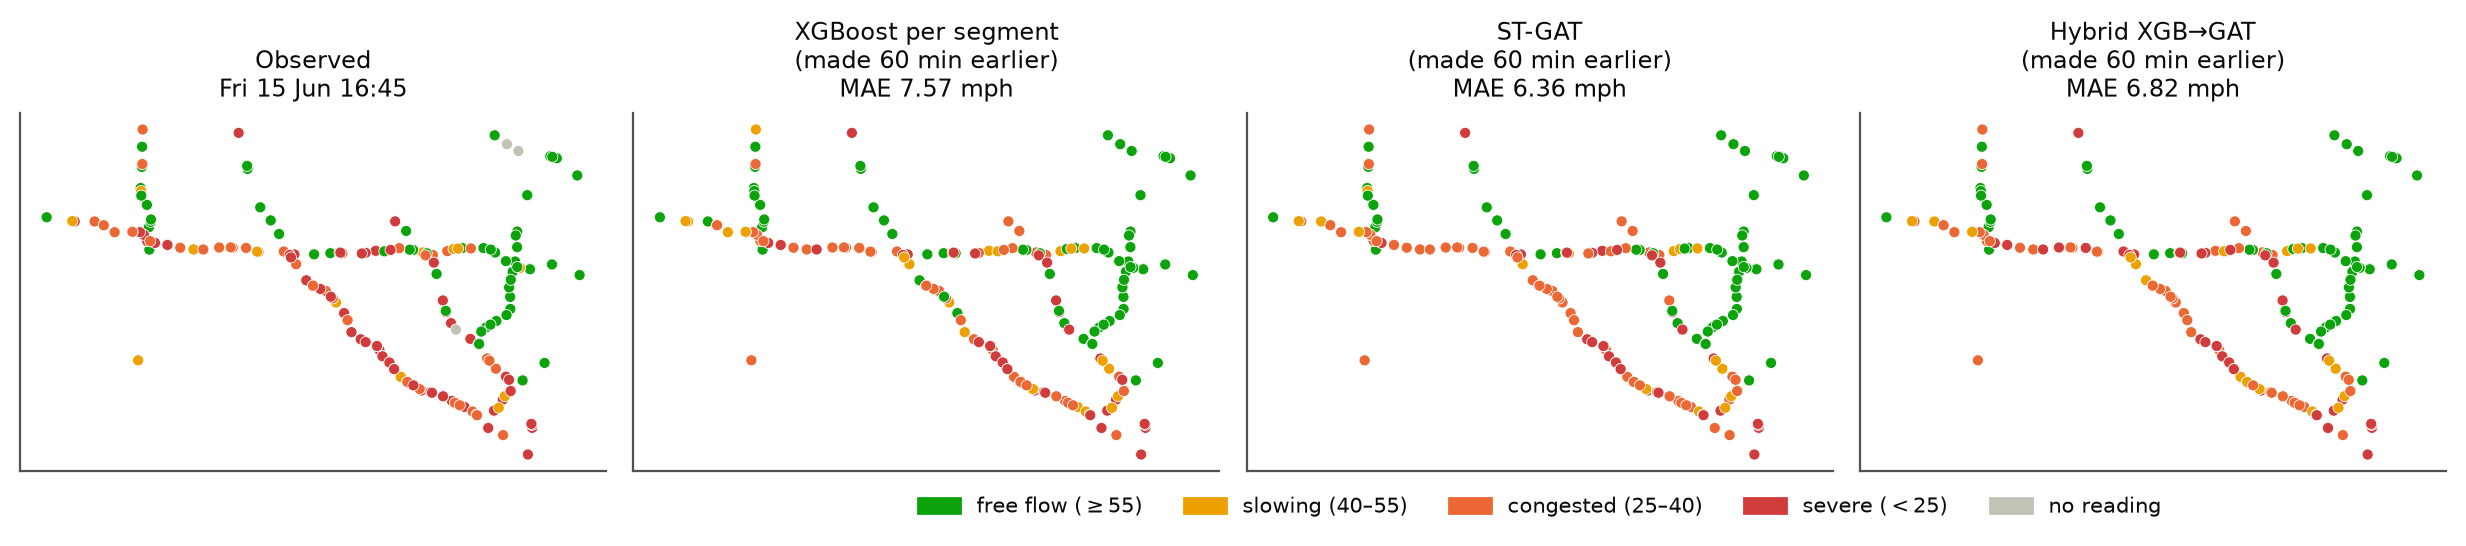
\includegraphics[width=0.95\textwidth]{p2_congestion_map.png}
\caption{Congestion map of the evening peak: observed speeds and 60-minute-ahead
forecasts of the per-segment, ST-GAT and hybrid models.}
\label{fig:congmap}
\end{figure*}

\begin{figure}[t]
\centering
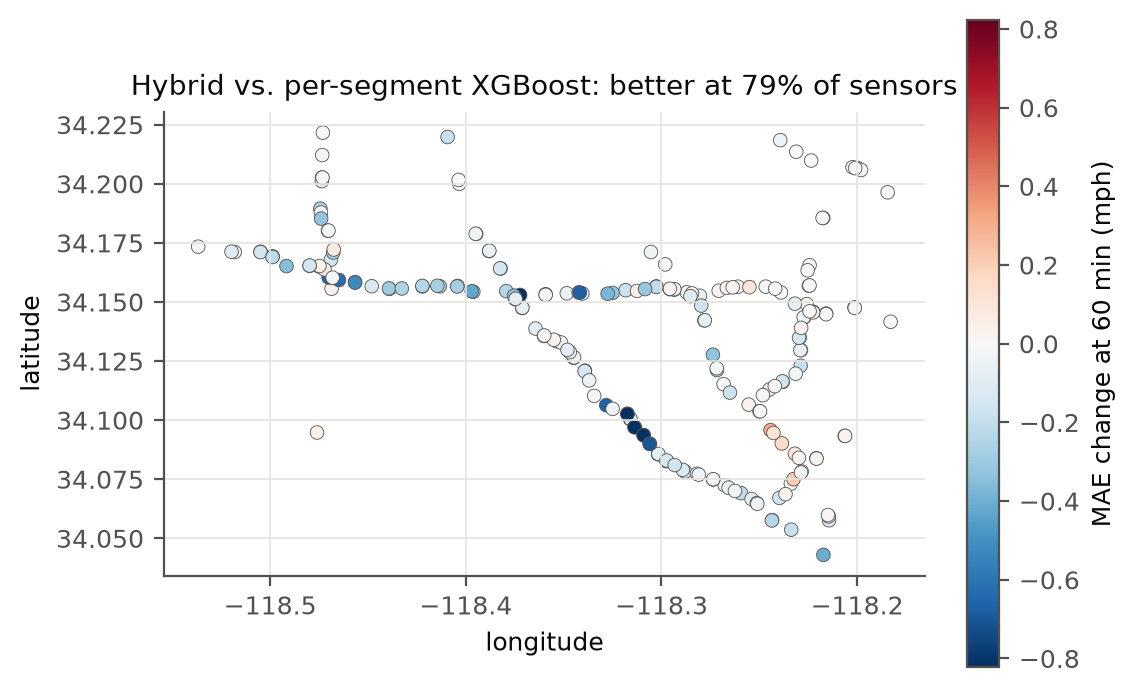
\includegraphics[width=0.9\columnwidth]{p2_improvement_map.png}
\caption{Per-sensor change in 60-minute MAE, hybrid minus XGBoost per segment
(blue: hybrid better).}
\label{fig:p2improve}
\end{figure}

The attention weights (Fig.~\ref{fig:attn}) are far from self-only: on average 84\,\%
of the attention mass goes to neighbours. The mass on neighbours rises when the
sensor is congested (downstream heads 0.84$\to$0.87, upstream 0.83$\to$0.87). The
shift is in the expected direction but small, consistent with the ``static'' ranking
of GAT attention~\cite{brody2022gatv2}, so we do not over-interpret the coefficients.

\begin{figure*}[t]
\centering
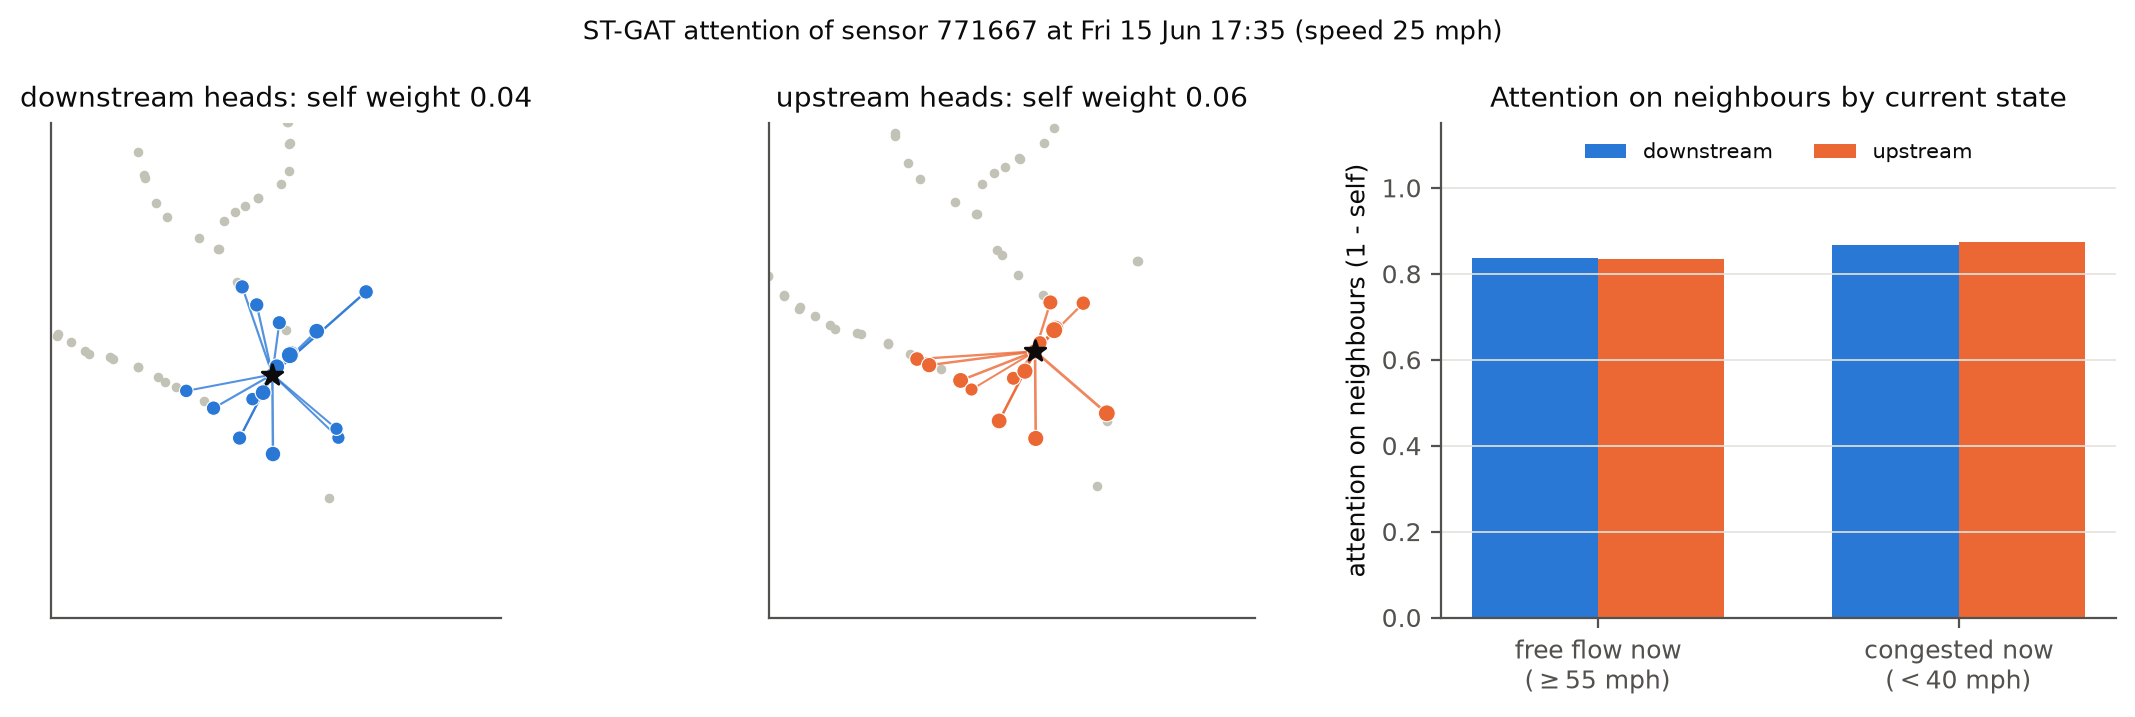
\includegraphics[width=0.9\textwidth]{p2_attention.png}
\caption{ST-GAT attention of one congested sensor during the evening peak
(downstream and upstream heads, first block), and the average attention on
neighbours by the sensor's current state.}
\label{fig:attn}
\end{figure*}

\subsection{Simulated signal-plan switching}
\begin{table}[t]
\centering
\caption{Simulated congestion-plan switching on the test period (6,554 congestion onsets). Offline replay only; no live control.}
\label{tab:p2signal}
\setlength{\tabcolsep}{3.5pt}
\begin{tabular}{lcccc}
\toprule
Policy & Antic.\,\% & Lead (min) & False\,\% & Switch/day \\
\midrule
Reactive (speed now) & 0.0 & 0 & 10.6 & 6.6 \\
XGBoost per segment & 19.8 & 10 & 7.7 & 4.1 \\
Graph WaveNet & 39.2 & 10 & 5.9 & 3.8 \\
ST-GAT & 30.1 & 10 & 7.7 & 3.4 \\
Hybrid XGB$\to$GAT & 35.7 & 10 & 6.0 & 3.8 \\
Oracle (true future) & 100.0 & 15 & 0.0 & 6.9 \\
\bottomrule
\end{tabular}
\end{table}
Table~\ref{tab:p2signal} replays the test period offline: a controller per sensor
switches to a congestion plan when it expects $<$40\,mph in 15\,minutes. A reactive
controller cannot anticipate any onset by construction. With forecasts, the plan is
already on 5--30 minutes before 20\,\% (XGBoost per segment) to 39\,\% (Graph
WaveNet) of the 6,554 congestion onsets, with a median lead time of 10\,minutes, while
false activations and plan switches fall compared with reactive control (e.g.\
10.6\,\%$\to$6.0\,\% false and 6.6$\to$3.8 switches per sensor-day for the hybrid).
The network models anticipate 1.5--2 times as many onsets as the independent model.
These are statements about \emph{decision timing} only: METR-LA has no turning
movements or signal timings, so we make no claim about delay, throughput or live
control.

\subsection{Training behaviour}
Fig.~\ref{fig:curves} shows the learning curves. ST-GAT's validation MAE is below its
training MAE throughout (dropout is active in training) and flattens after about 30
epochs; two learning-rate halvings give small further gains. The hybrid starts at the
XGBoost forecast, improves validation MAE from 3.03 to 2.87\,mph within 25 epochs and
then plateaus while its training MAE keeps falling (2.76$\to$2.70), a sign that the
correction network begins to fit noise in the residuals; early stopping keeps the
best validation checkpoint.

\begin{figure}[t]
\centering
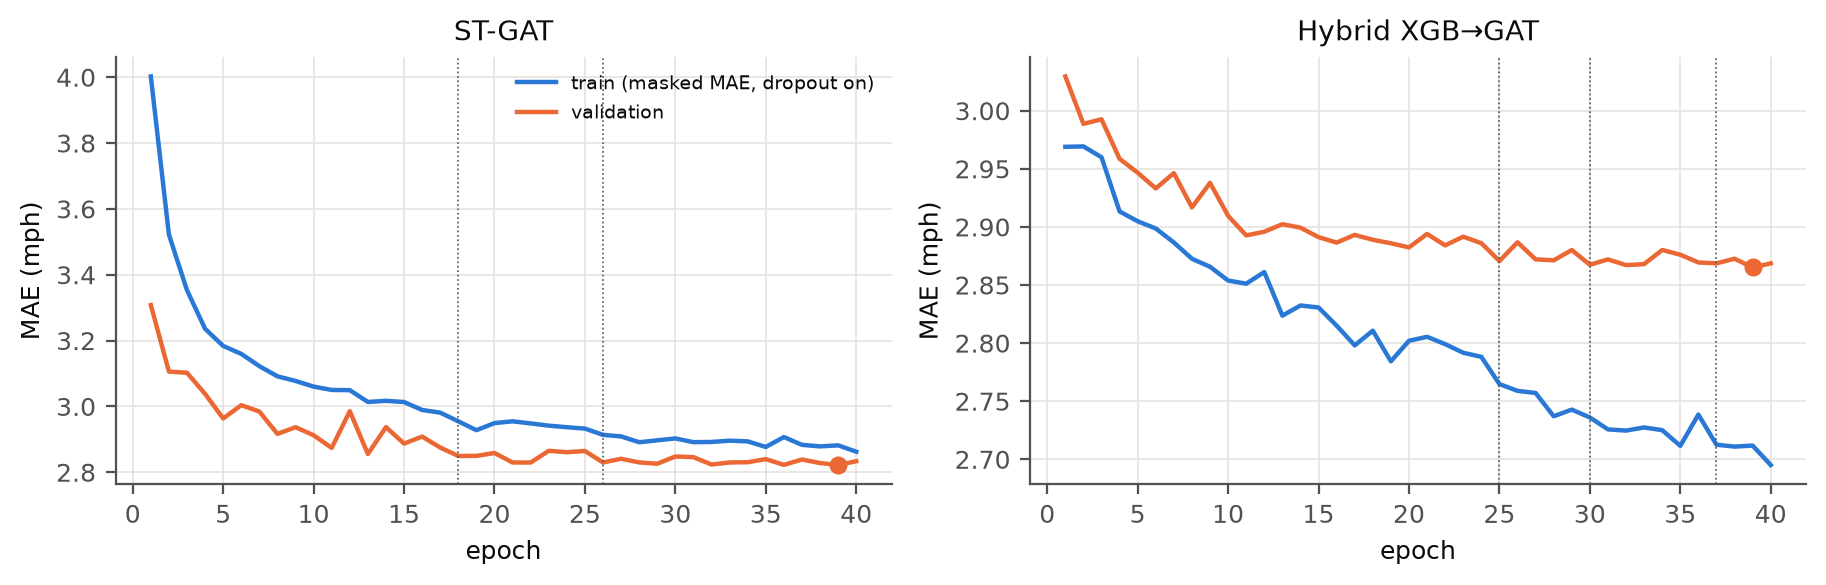
\includegraphics[width=\columnwidth]{p2_learning_curves.png}
\caption{Learning curves of the two main Phase~2 runs (dots: best validation epoch;
dotted lines: learning-rate halvings).}
\label{fig:curves}
\end{figure}
